\chapter{Implementasi dan Pengujian}
\label{chap:implementasiPengujian}

Bab ini berisi Implementasi Perangkat Lunak dan Pengujian Perangkat Lunak. Bagian implementasi terdiri dari penjelasan lingkungan pengembangan perangkat lunak dan hasil implementasi. Bagian pengujian terdiri dari hasil pengujian fungsional dan eksperimental terhadap perangkat lunak yang
telah dibangun.

\section{Implementasi}
\label{sec:implementasi} 

\subsection{Lingkungan Implementasi}
\label{sec:lingkunganImplementasi}

Implementasi perangkat lunak ini dilakukan pada komputer penulis dengan spesifikasi berikut:

\begin{enumerate}
	\item \textit{Processor}: AMD Ryzen 7 4800H
	\item \textit{Random Access Memory} (RAM): 8 GB DDR4
	\item Sistem Operasi: Windows 11
\end{enumerate}

\subsection{Hasil Implementasi}
\label{sec:hasilImplementasi}

Terdapat dua hasil implementasi, yaitu :

\begin{enumerate}
	\item Sebuah halaman formulir data umat baru yang memiliki fitur responsif (terbaca mudah di ponsel), berisikan formulir SIMU (Sistem Informasi Manajemen Umat), data dapat tersimpan pada lokal, membangkitkan kode QR  yang nantinya dapat dibaca oleh Odoo.
	\item Sistem Odoo yang berisi data yang field-field nya menyerupai data umat SIMU (Sistem Informasi Manajemen Umat) dan mampu memindai kode QR yang dihasilkan dari halaman formulir data umat baru. 
\end{enumerate}

\section{Tampilan Antarmuka}
\label{sec:tampilanAntarMuka}

\subsection{Tampilan Antarmuka Formulir Data Umat}
\label{sec:tampilanAntarmukaFormulir}

\begin{figure}[H]
	\centering
	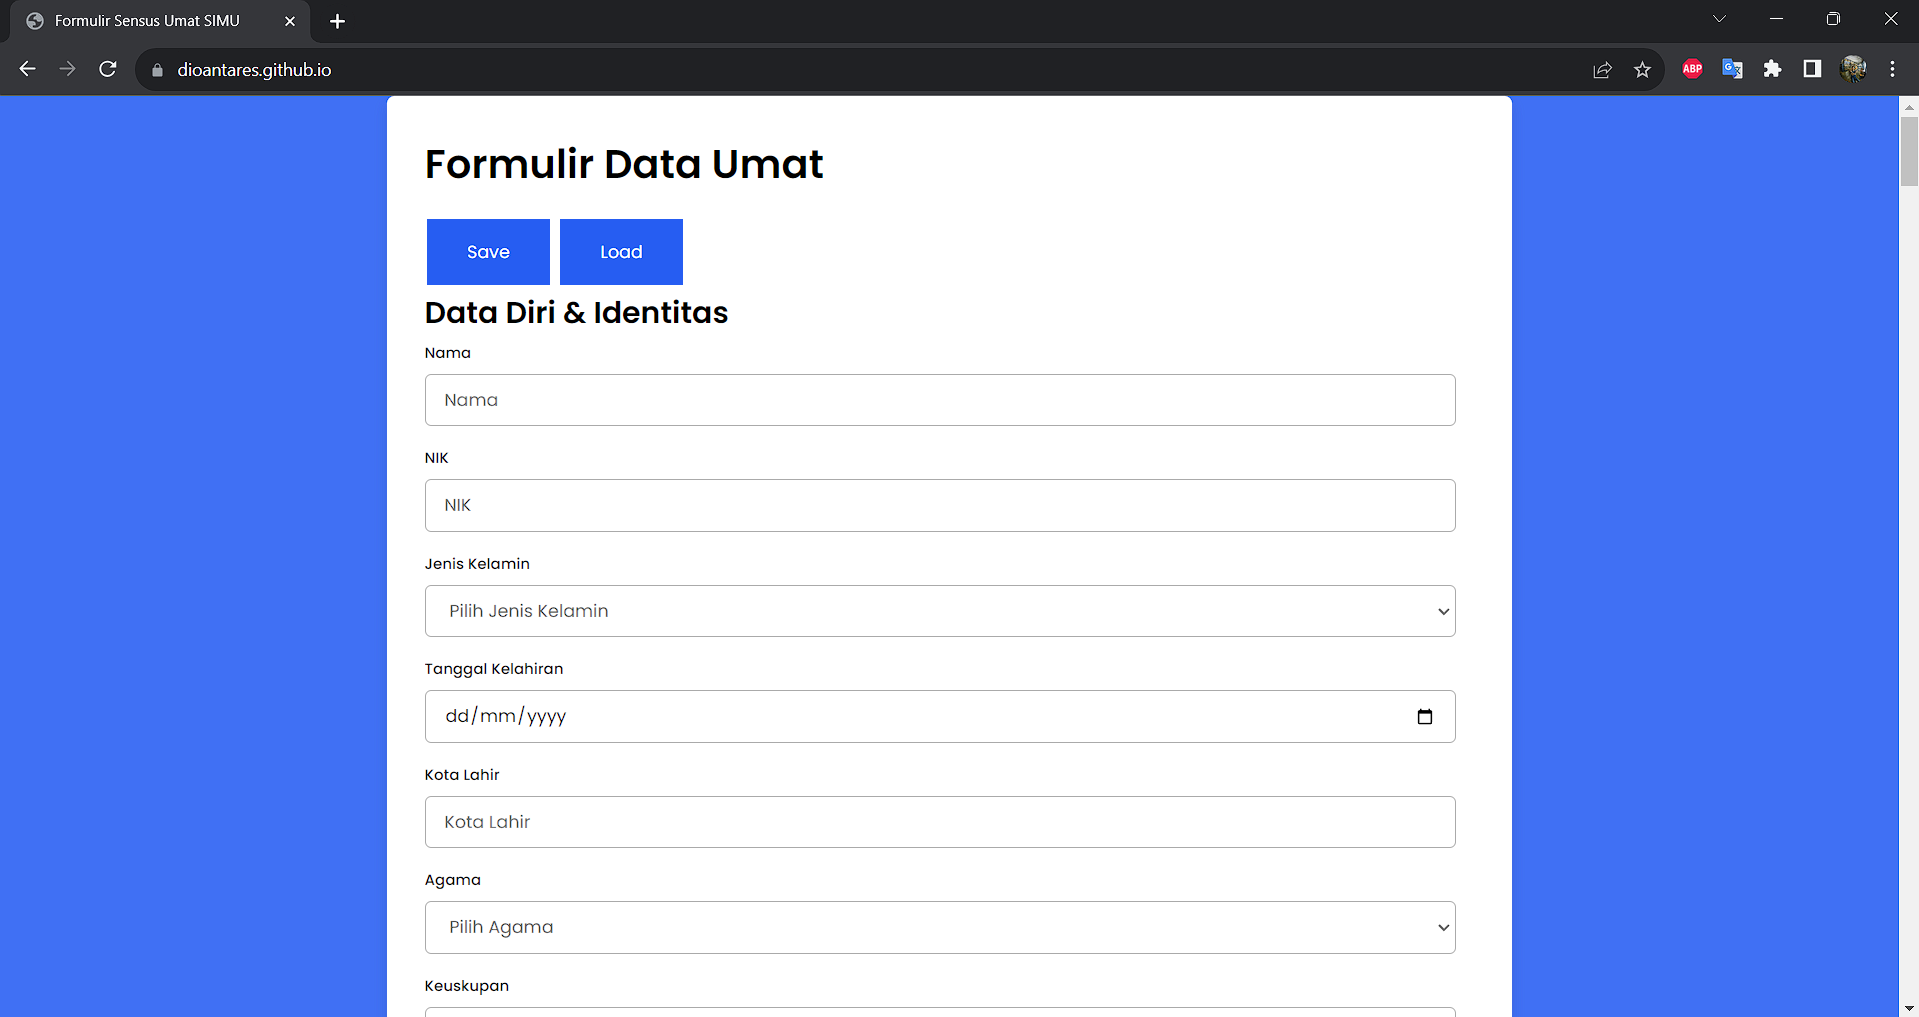
\includegraphics[scale=0.4]{Gambar/halamanFormulir.png}
	\caption{Hasil implementasi antarmuka halaman Formulir Data Umat} 
	\label{fig:formDataUmatFull}
\end{figure}

Umat yang akan mendaftar dapat mengakses website tersebut melalui link \url{https://dioantares.github.io/}. Gambar \ref{fig:formDataUmatFull} merupakan tampilan antarmuka pada halaman Formulir Data Umat yang sudah diimplementasikan. File \textit{style} dan \textit{script} untuk halaman ini terletak di file terpisah.  Apabila umat sudah selesai menyelesaikan pengisian formulir data umat, maka pada bagian bawah halaman website akan terdapat tombol submit, seperti pada gambar \ref{fig:fiturSubmit}.

\begin{figure}[H]
	\centering
	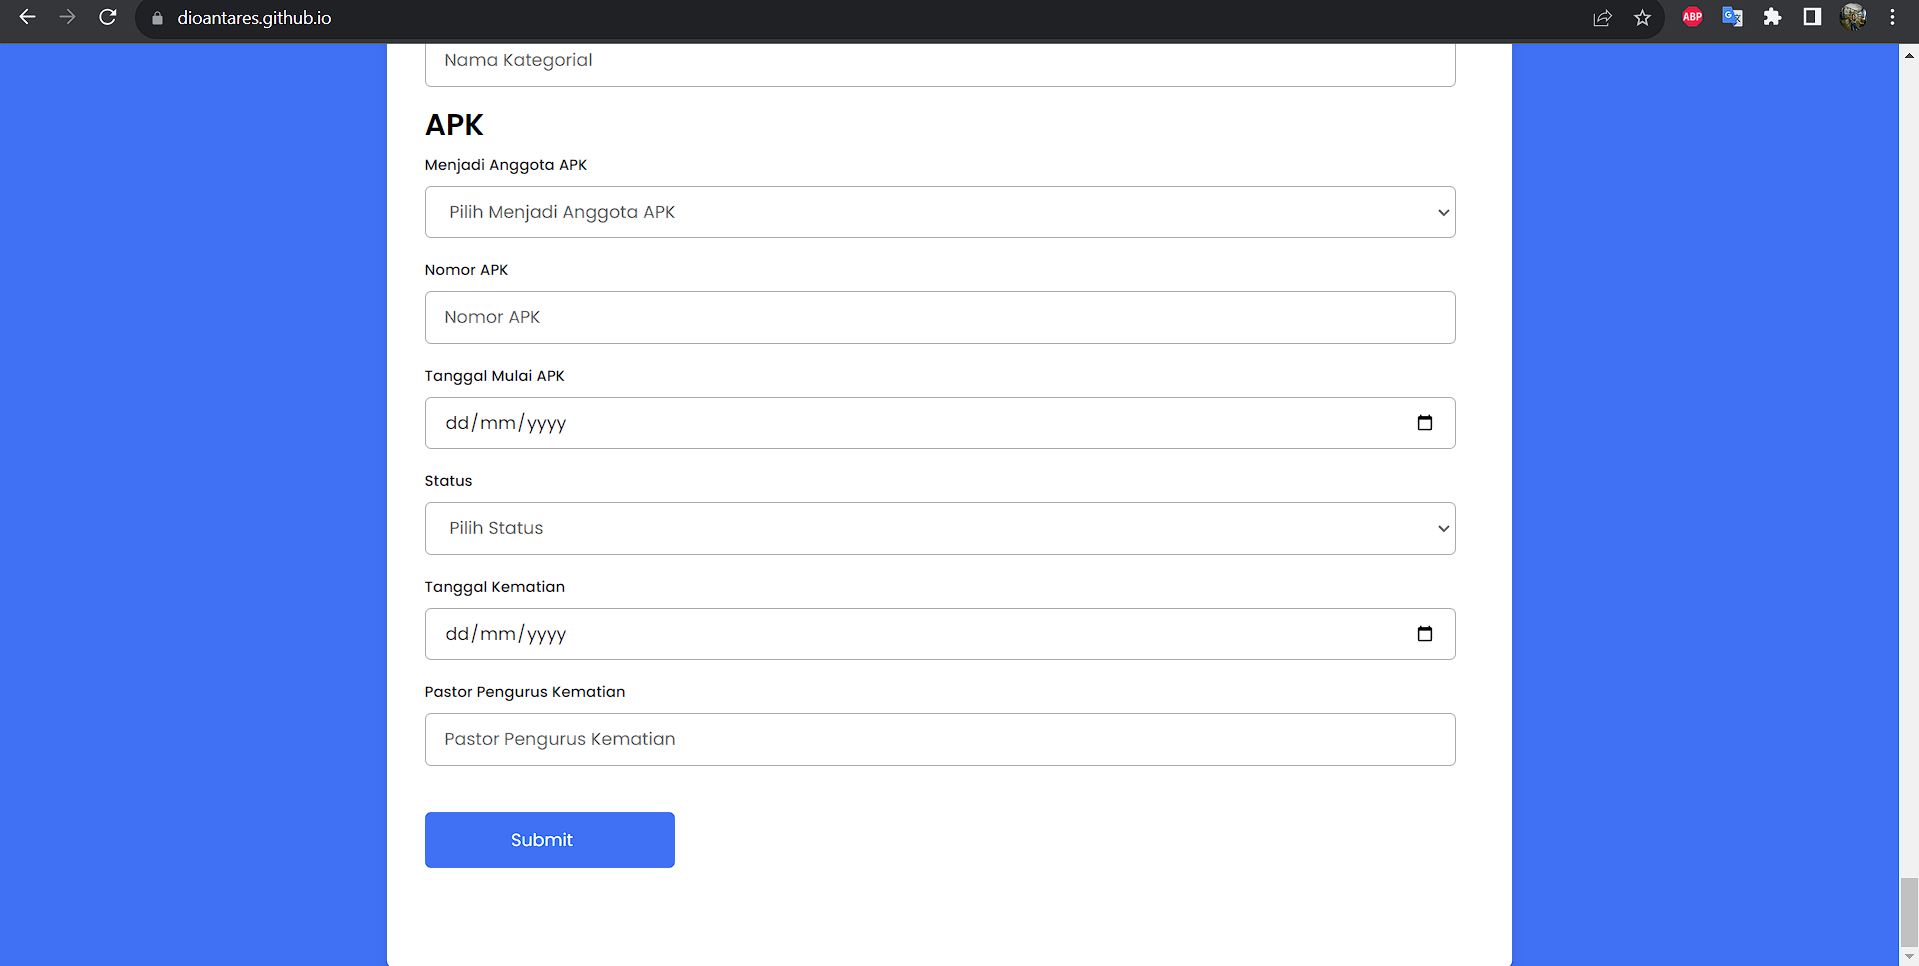
\includegraphics[scale=0.4]{Gambar/fiturSubmit.png}
	\caption{Hasil implementasi fitur submit pada website formulir data umat} 
	\label{fig:fiturSubmit}
\end{figure}

Setelah data umat selesai terisi, dan umat menekan tombol submit, maka proses selanjutnya adalah website akan merubah data yang terisi pada field input formulir menjadi sebuah qr code, maka halaman website akan menampilkan qr code yang sudah berisikan data yang telah ditulis pada field input formulir, seperti pada gambar \ref{fig:contohQRCodeSubmit}.

\begin{figure}[H]
	\centering
	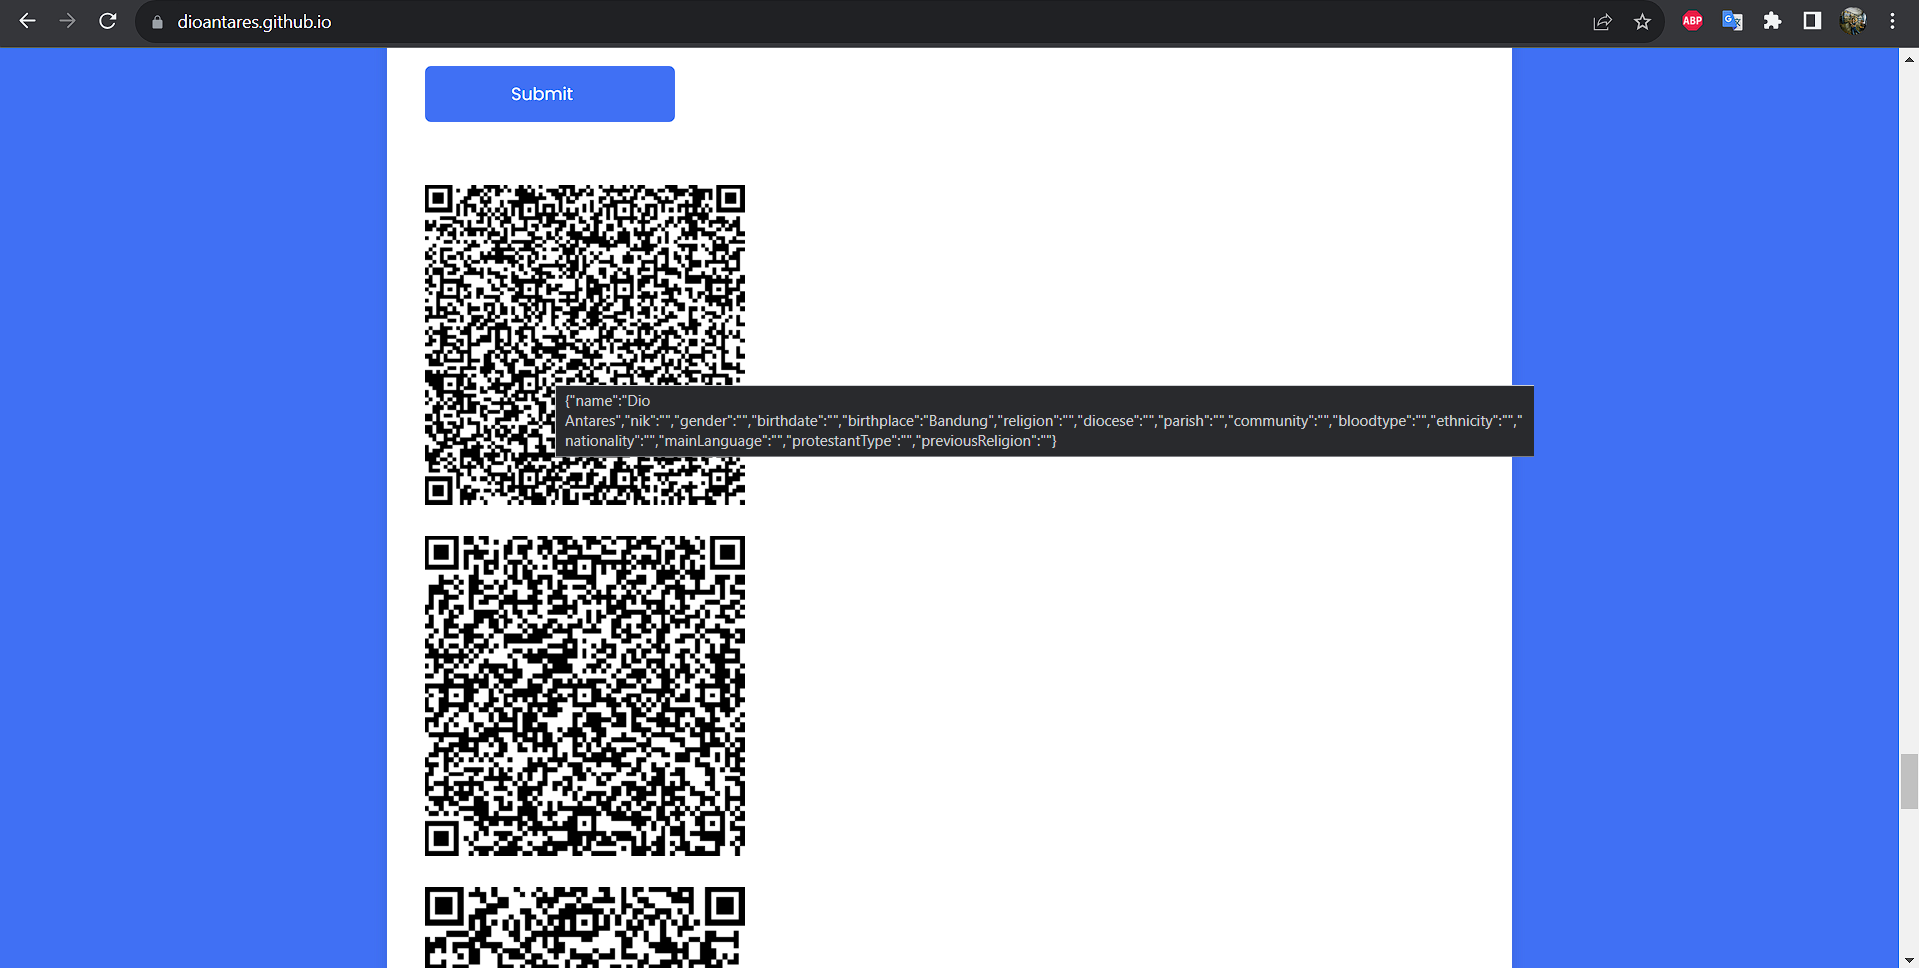
\includegraphics[scale=0.4]{Gambar/contohQRCodeSubmit.png}
	\caption{Hasil implementasi contoh QR Code yang berhasil ditampilkan} 
	\label{fig:contohQRCodeSubmit}
\end{figure}

Pada gambar \ref{fig:contohQRCodeSubmit}, apabila qr code sudah berhasil ditampilkan, maka umat hanya perlu menunjukkannya kepada admin, sehingga admin dapat mempindai qr code tersebut. Pengisian formulir data umat baru dilakukan secara online sehingga dapat mengurangi waktu penulisan data umat baru dan mengurangi kemungkinanan kesalahan dalam penulisan data umat baru, selain itu dengan adanya halam website ini maka umat dapat menggunakan fitur save dan load, fitur ini berfungsi apabila umat baru akan melanjutkan pengisian formulir dilain waktu, atau mencegah terjadinya \textit{crash} pada halaman website, sehingga umat tidak perlu menulis ulang dari awal apabila terjadi hal yang tidak diinginkan. Pemberitahuan apabila save berhasil maka akan menampilkan notifikasi "Data Berhasil di Save", seperti pada gambar \ref{fig:saveBerhasil} dan apabila load berhasil maka akan menampilkan notifikasi "Data Berhasil di Load", seperti pada gambar \ref{fig:loadBerhasil}. Tombol save dan load berada pada bagian atas halaman website, contohnya dapat dilihat pada gambar \ref{fig:formDataUmatFull}.

\begin{figure}[H]
	\centering
	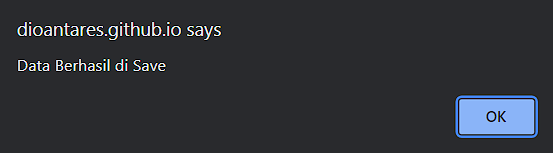
\includegraphics[scale=0.4]{Gambar/saveBerhasil.png}
	\caption{Hasil implementasi fitur notifikasi data berhasil di save} 
	\label{fig:saveBerhasil}
\end{figure}

\begin{figure}[H]
	\centering
	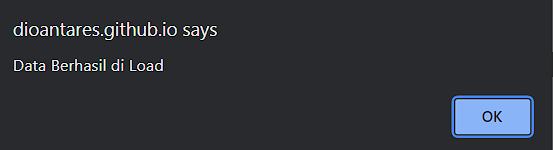
\includegraphics[scale=0.4]{Gambar/loadBerhasil.png}
	\caption{Hasil implementasi fitur notifikasi data berhasil di load} 
	\label{fig:loadBerhasil}
\end{figure}

\begin{figure}[H]
	\centering
	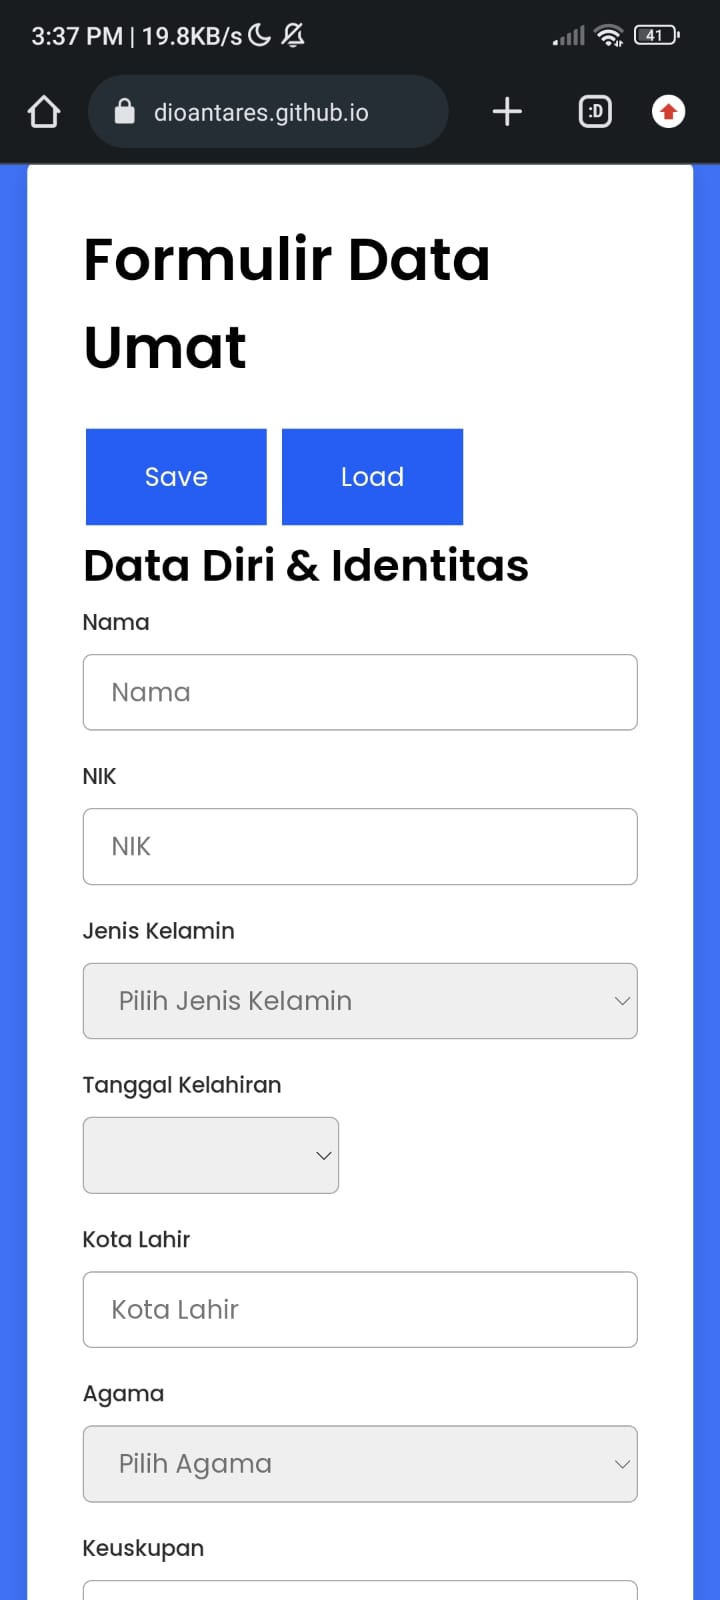
\includegraphics[scale=0.3]{Gambar/websiteHP.jpg}
	\caption{Hasil implementasi antarmuka halaman Formulir Data Umat pada Handphone} 
	\label{fig:websiteHP}
\end{figure}

Pada gambar \ref{fig:websiteHP} menunjukan bahwa website formulir data umat berhasil dimplementasikan secara responsif, sehingga tampilan website tidak berubah apabila dibuka diberbagai \textit{device}.

\subsection{Tampilan Antarmuka Odoo}
\label{sec:tampilanAntarmukaOdoo}

Pada pembuatan tampilan antarmuka Odoo, sudah berhasil membuat module custom Odoo, namun untuk fitur yang dibutuhkan masih terdapat kesulitan untuk menyempurnakan fitur tersebut. Terdapat dua cara yang dilakukan, yaitu dengan membuat halaman yang berisikan field data umat, dan cara yang kedua yaitu dengan membuat halaman custom menggunakan controller pada Odoo.

\begin{figure}[H]
	\centering
	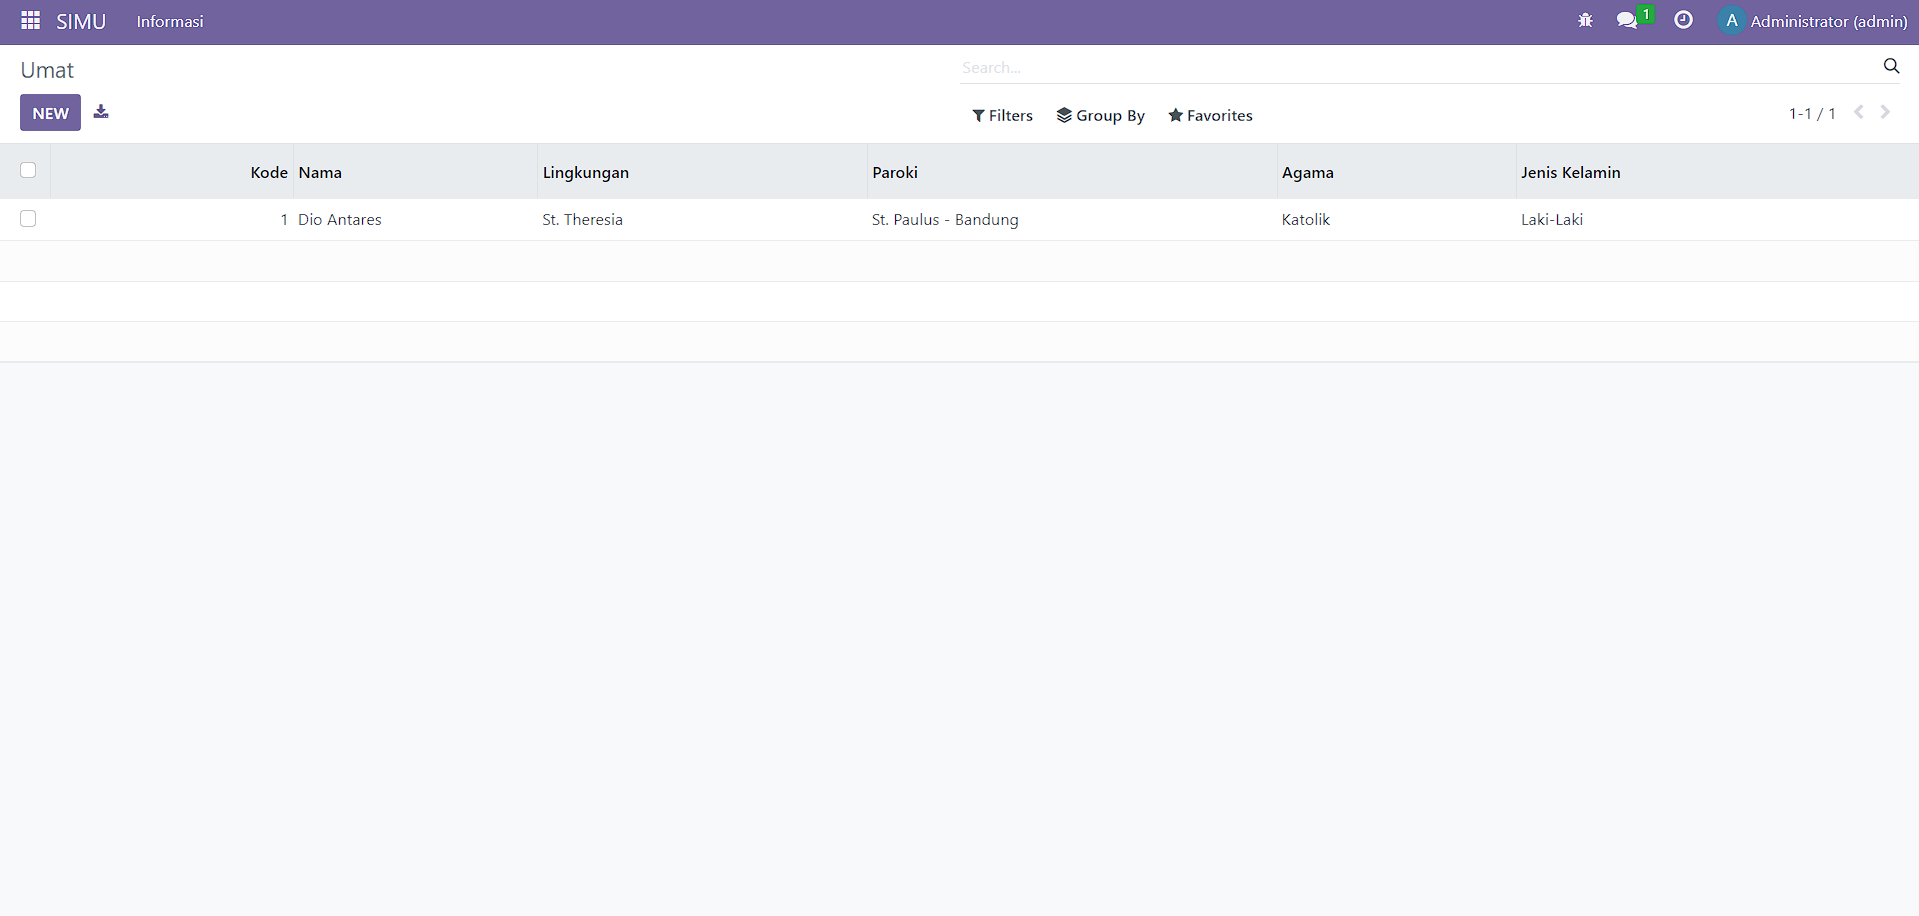
\includegraphics[scale=0.4]{Gambar/odooBuatBaru.png}
	\caption{Hasil implementasi antarmuka halaman Odoo} 
	\label{fig:odooBuatBaru}
\end{figure}

Gambar \ref{fig:odooBuatBaru} adalah halaman custom module Odoo yang sudah berhasil dibuat, untuk mengakses halaman tersebut maka penulis harus membuka halaman melalui link \url{http://localhost:8069/web}, halaman tersebut hanya dapat diakses melalui file local yang sudah berhasil menginstall custom module Odoo pada perangkat yang digunakan.

\begin{figure}[H]
	\centering
	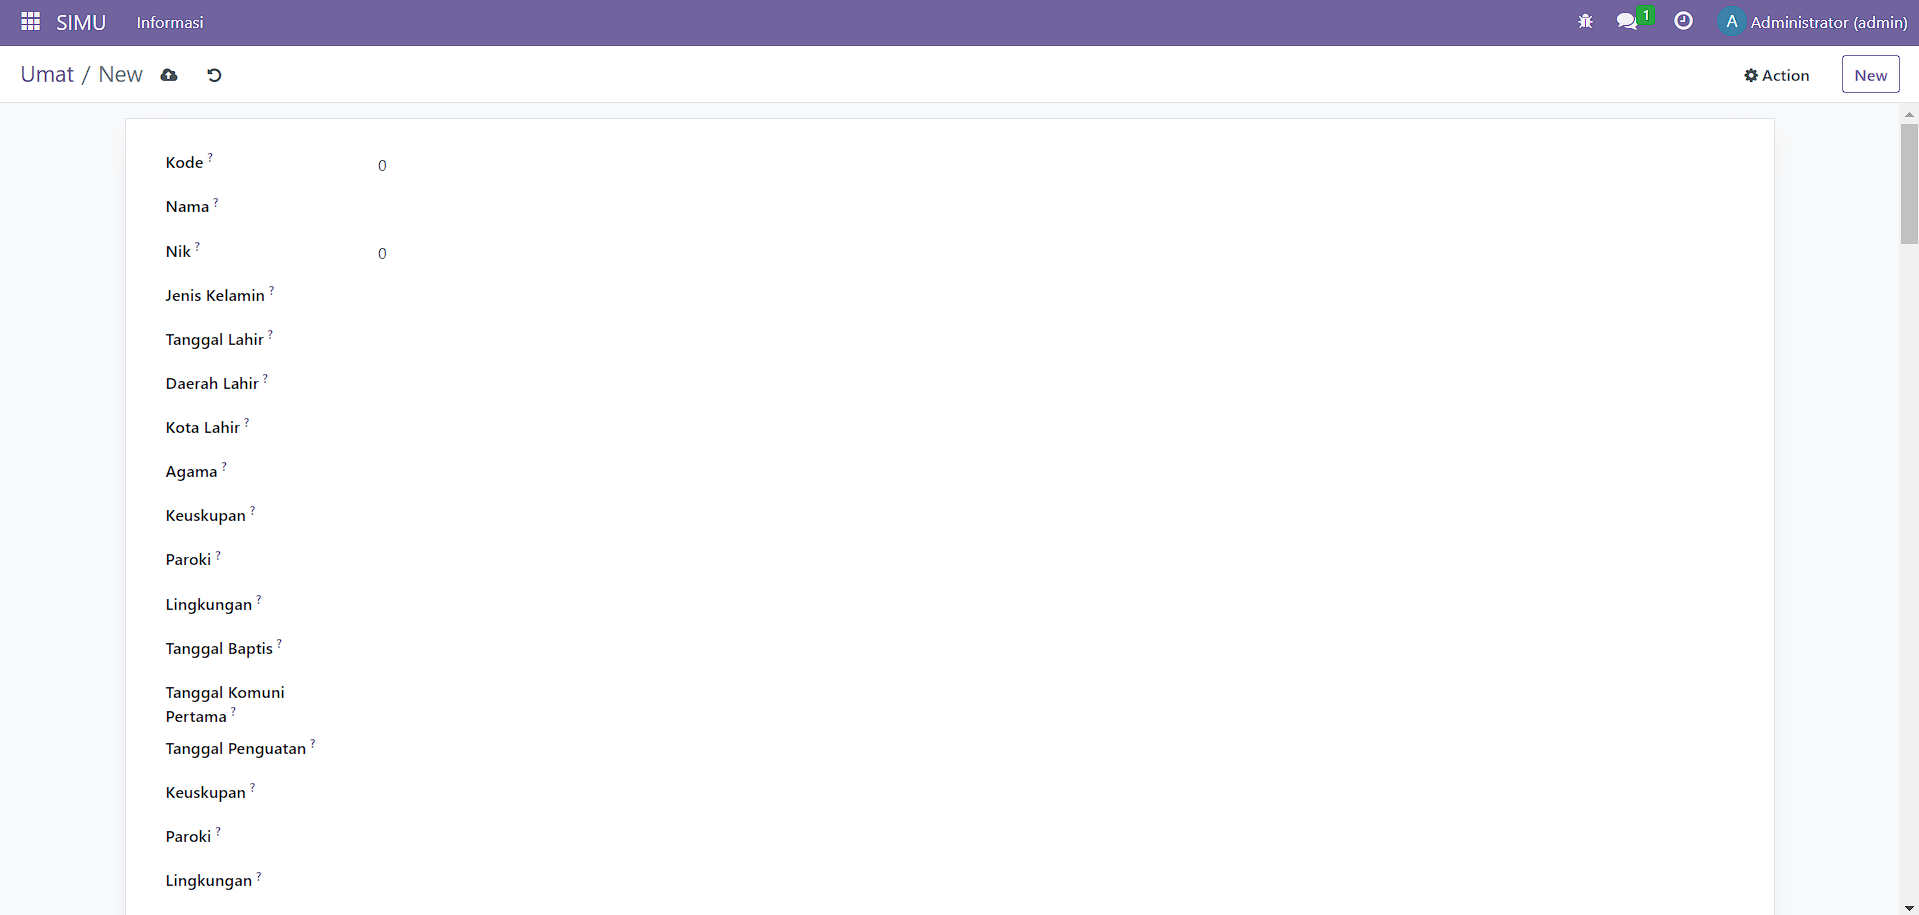
\includegraphics[scale=0.4]{Gambar/odooBuatBaru2.png}
	\caption{Hasil implementasi antarmuka halaman Odoo untuk submit} 
	\label{fig:odooBuatBaru2}
\end{figure}

Gambar \ref{fig:formDataUmatFull} merupakan tampilan antarmuka pada halaman Formulir Data Umat yang sudah diimplementasikan, sedangkan pada gambar \ref{fig:odooBuatBaru} merupakan halaman utama yang menampilkan data umat, lalu pada gambar \ref{fig:odooBuatBaru2} merupakan halaman odoo yang berfungsi untuk menambahkan data umat baru, untuk menuju halaman ini, admin perlu menakan tombol \textit{New} pada pojok kiri atas halaman utama.

\begin{figure}[H]
	\centering
	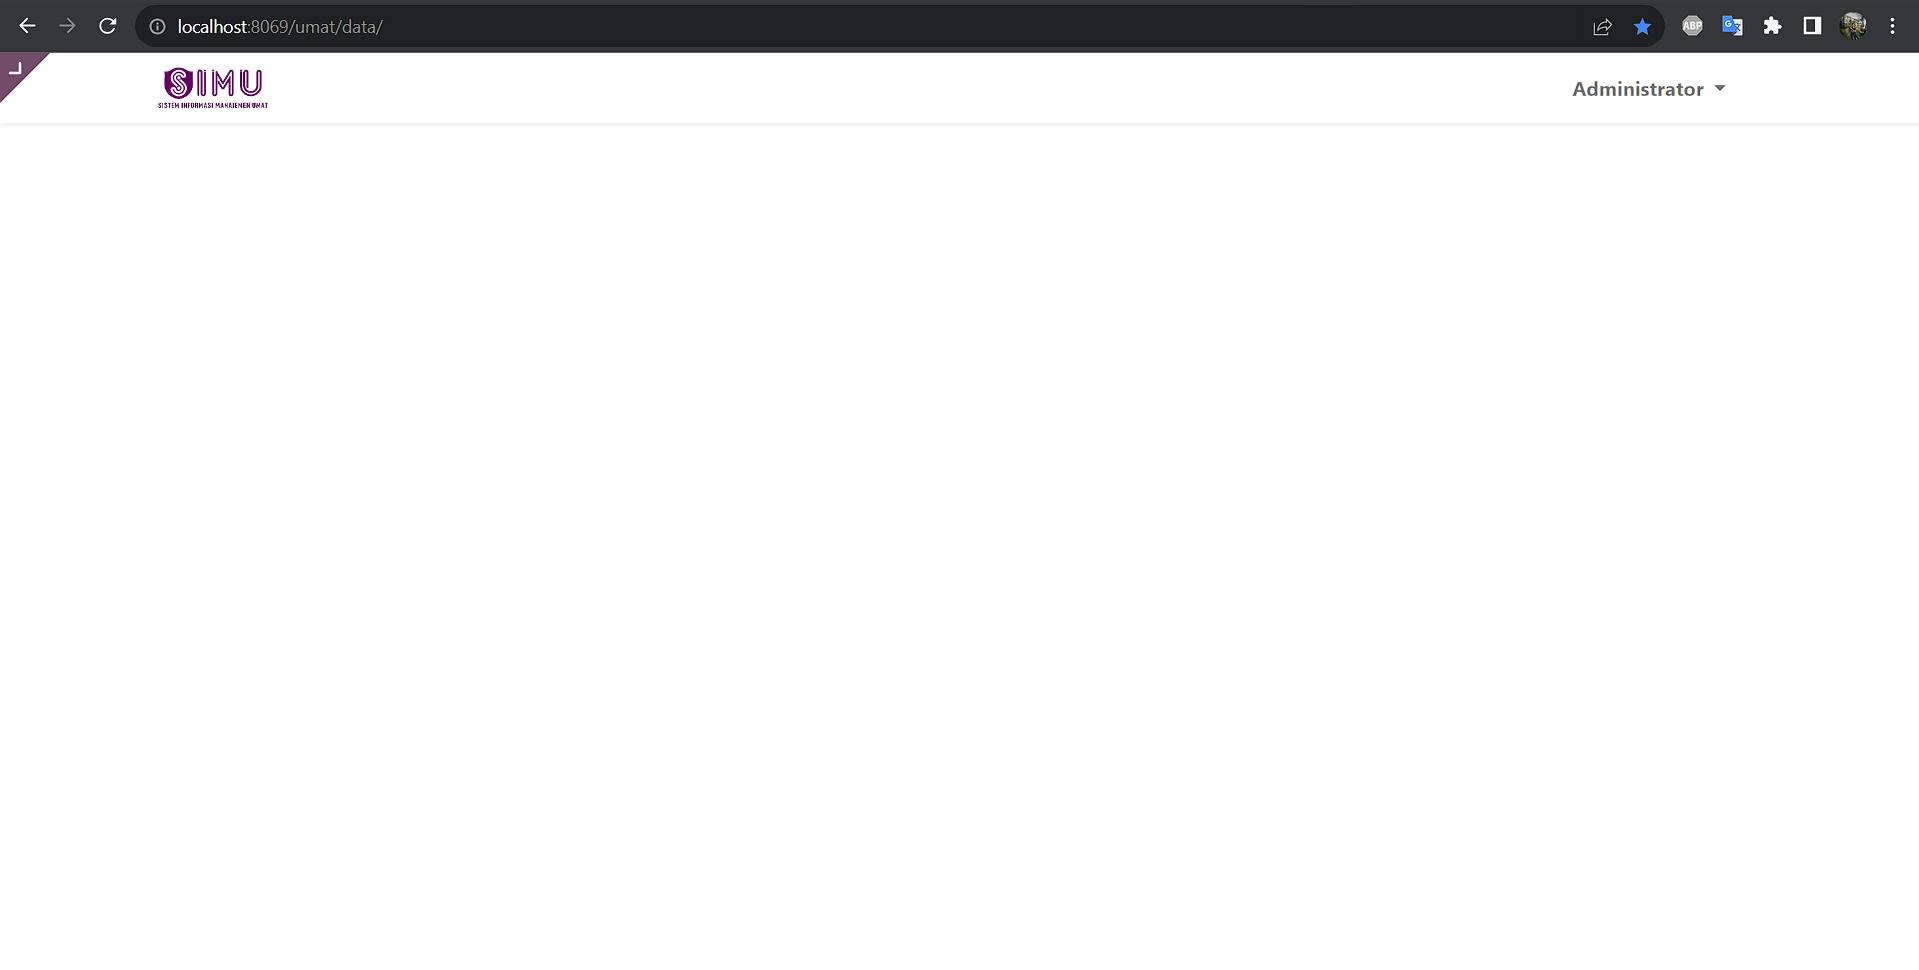
\includegraphics[scale=0.4]{Gambar/controllerOdoo.png}
	\caption{Hasil pembuatan halaman html pada Odoo} 
	\label{fig:controllerOdoo}
\end{figure}

Telah dilakukan pengujian terhadap custom halaman Odoo menggunakan Controller, cara ini dilakukan dengan cara membuat halaman baru, dengan url yang sudah kita tentukan sendiri. Contoh pembuatan halaman html custom pada odoo terdapat pada gambar \ref{fig:controllerOdoo} merupakan tampilan halaman website yang berfungsi untuk memindai QR Code, namun halaman ini baru berhasil menampilkan dan membuka camera webcam. Cara ini dilakukan karena pada saat membuat halaman custom pada Odoo langsung cukup sulit.

\section{Pengujian Fungsional}
\label{sec:pengujianFungsional}

Pengujian fungsional dilakukan secara lokal pada perangkat penulis. Berikut ini pengujian yang dilakukan terhadap fitur-fitur yang sudah diimplementasi:

\subsection{Pengujian Fungsional Formulir Data Umat Baru}
\label{sec:pengujianFungsionalFormulir}

\begin{table}[H]
	\centering
	\caption{Tabel Pengujian Fungsional Formulir Data Umat Baru}
	\begin{tabular}{|p{0.5cm}| p{5cm}| p{6cm}| p{2.5cm}|} \hline
		No	&	Aksi Pengguna	&	Reaksi yang diharapkan	&	Reaksi \\ \hline
		1 	&  Membuka halaman utama & Halaman formulir ditampilkan &	sesuai	\\ \hline
		2 	&  Membuka halaman pada ponsel & Responsif (terbaca mudah di ponsel) &	sesuai	\\ \hline
		3 	&  Mengetik data pada form yang tersedia & Menampilkan keyboard yang tepat untuk input tertentu (contoh: nomor telepon menggunakan keypad) &	sesuai	\\ \hline
		4 	&  Menekan tombol save & Data disimpan ditandai dengan \textit{status} "Data Berhasil di Save" &	sesuai	\\ \hline
		5 	&  Menekan tombol Load & Data diload ditandai dengan \textit{status} "Data Berhasil di Load" &	sesuai	\\ \hline
		6 	&  Menekan tombol Submit & Menampilkan kode QR sesuai dengan data yang telah diisi &	sesuai	\\ \hline
	\end{tabular}
	\label{table:fungsionalFormulir}
\end{table}

\subsection{Pengujian Fungsional Odoo}
\label{sec:pengujianFungsionalOdoo}

\begin{table}[H]
	\centering
	\caption{Tabel Pengujian Fungsional Odoo}
	\begin{tabular}{|p{0.5cm}| p{5cm}| p{6cm}| p{2.5cm}|} \hline
		No	&	Aksi Pengguna	&	Reaksi yang diharapkan	&	Reaksi \\ \hline
		1 	&  Membuka halaman utama & Halaman utama ditampilkan &	sesuai	\\ \hline
		2 	&  Menekan tombol New & Menampilkan halaman dengan field data umat baru &	sesuai	\\ \hline
		3 	&  Membuka akses kamera & Membuka kamera &	sesuai	\\ \hline
		4 	&  Menekan tombol Scan & Mampu memindai kode QR  &	belum sesuai	\\ \hline
	\end{tabular}
	\label{table:fungsionalOdoo}
\end{table}

\section{Pengujian Eksperimental}
\label{sec:pengujianEksperimental}

Pengujian eksperimental dilakukan oleh \textit{handphone} penulis dengan spesifikasi sebagai berikut:

\begin{enumerate}
	\item \textit{Handphone}: Redmi Note 12
	\item \textit{Random Access Memory} (RAM): 8 GB
	\item Android: 13
\end{enumerate}

Pada pengujian eksperimental ini dilakukan dengan cara penulis melakukan pengisian formulir dengan tiga contoh kasus, yang pertama dengan \textit{average case} yaitu berisikan data asli penulis dan benar apa adanya, yang kedua adalah \textit{best case} yaitu berisikan data yang mencakup satu huruf saja untuk setiap fieldnya, yang ketiga adalah \textit{worst case} yaitu berisikan data yang cukup panjang pada setiap fieldnya. 

\subsection{Pengujian Average Case}
\label{sec:pengujianAverage}

Pada pengujian ini dilakukan menggunakan data asli penulis, hanya beberapa pengisian field dilakukan secara palsu atau tidak sesuai data penulis.


\begin{figure}[H]
	\centering
	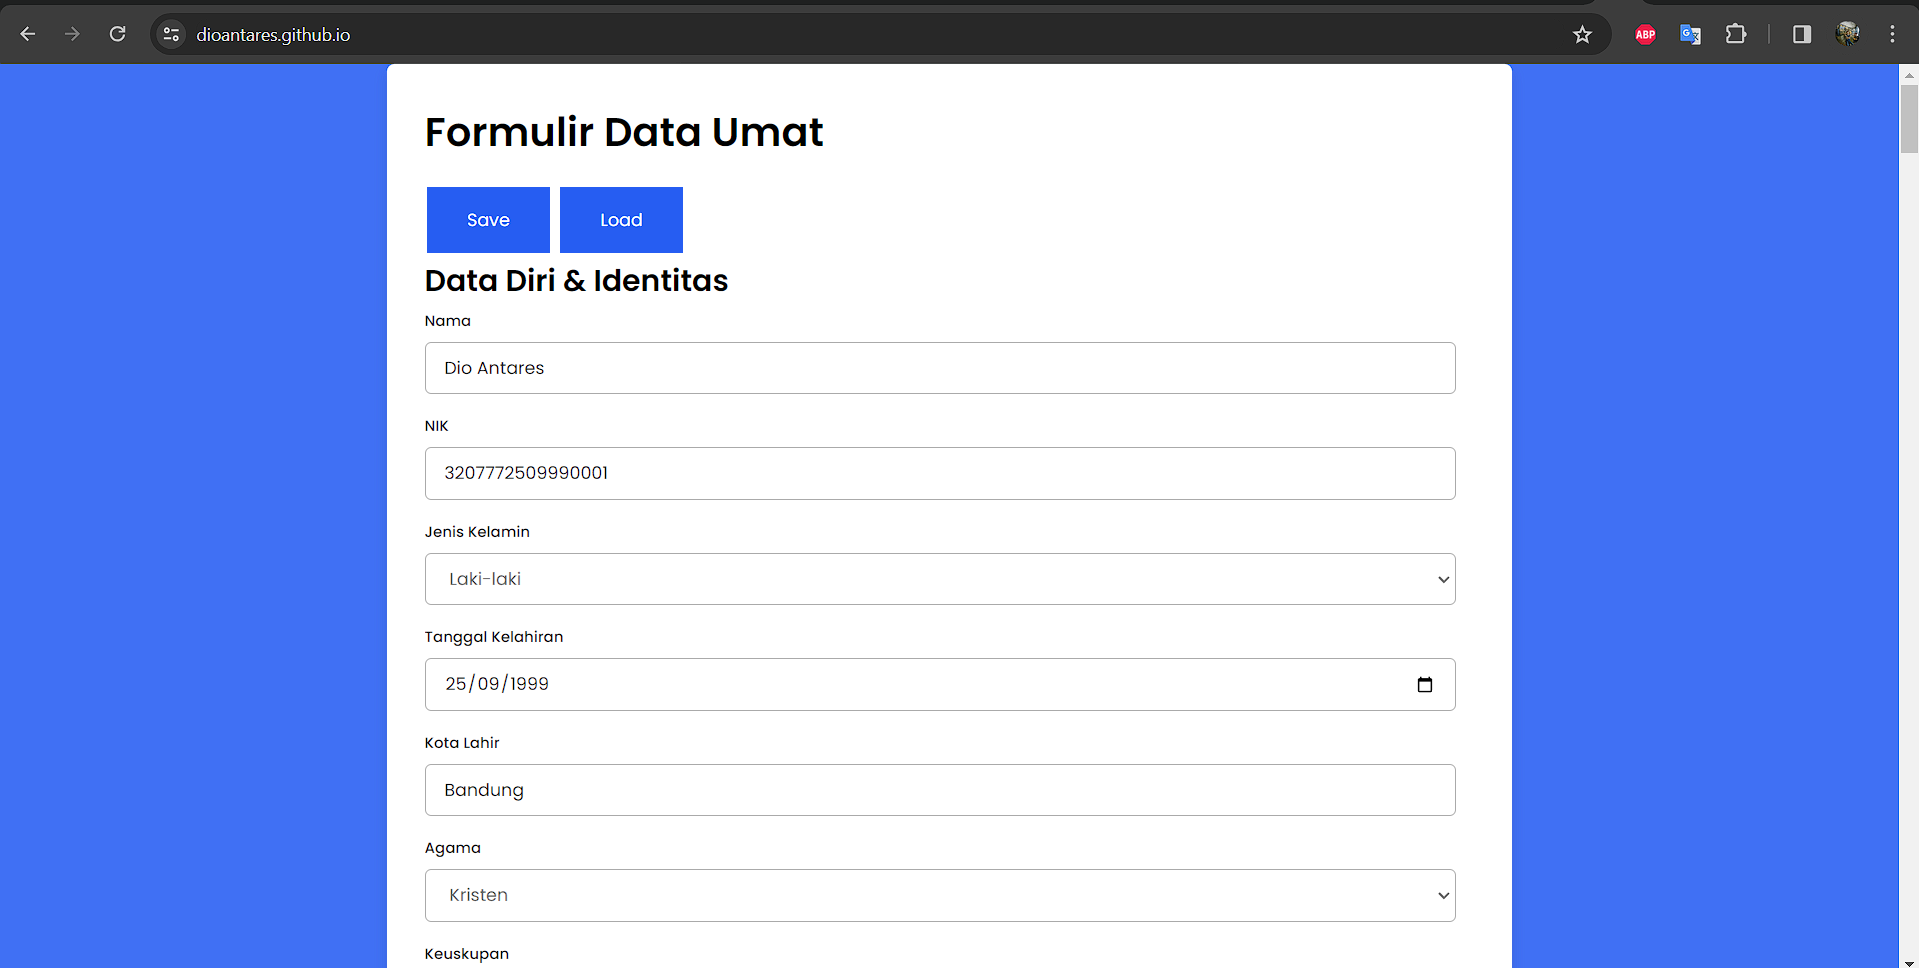
\includegraphics[scale=0.4]{Gambar/inputAverageCase.png}
	\caption{Input data average case pada data formulir} 
	\label{fig:inputAverageCase}
\end{figure}

\begin{figure}[H]
	\centering
	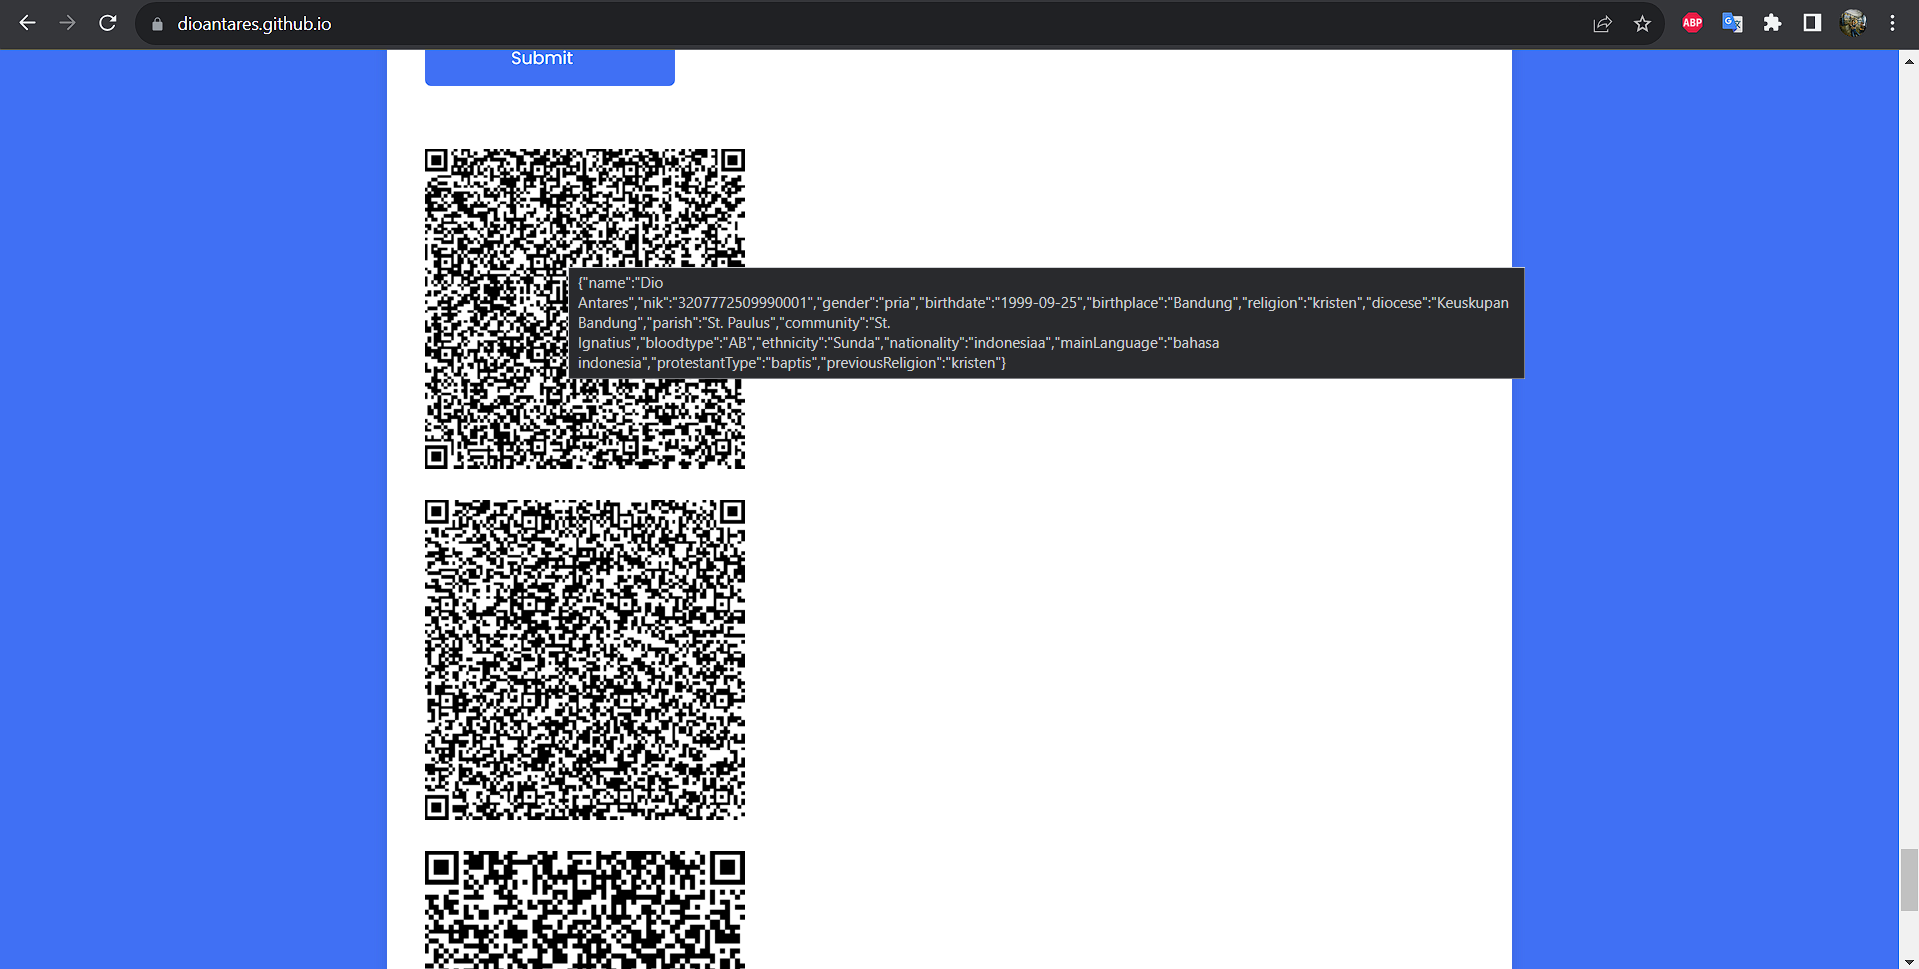
\includegraphics[scale=0.4]{Gambar/formFullQRCode.png}
	\caption{Hasil qr code average case dari data formulir} 
	\label{fig:formFullQRCode}
\end{figure}

\begin{figure}[H]
	\centering
	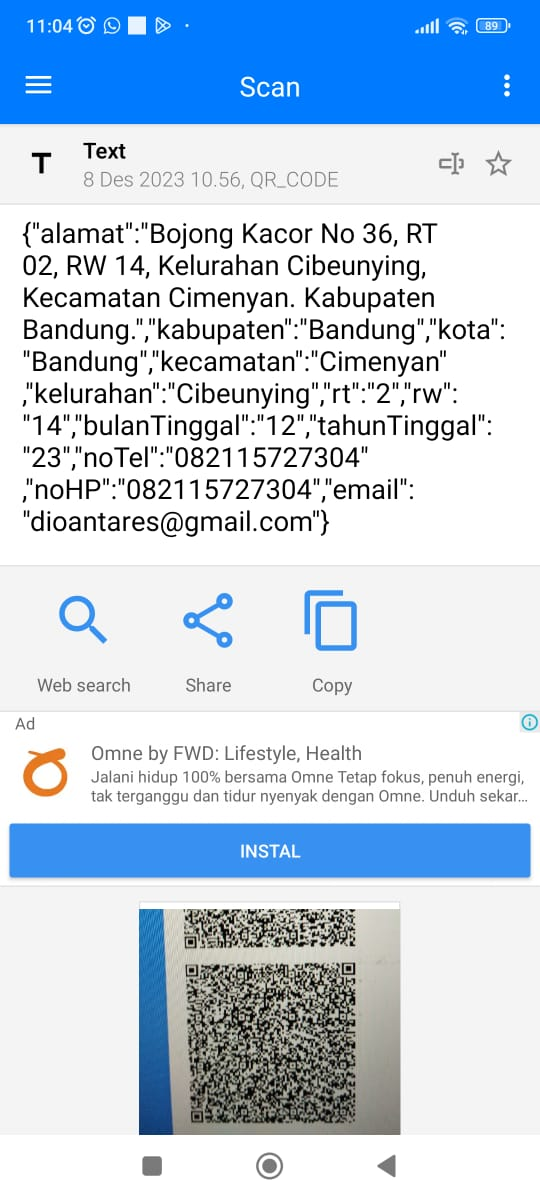
\includegraphics[scale=0.4]{Gambar/hasilScan.jpg}
	\caption{Hasil scan QR Code melalui aplikasi pada handphone} 
	\label{fig:hasilScan}
\end{figure}

Hasil pengujian ini mendapatkan hasil yang bagus, terbukti pada gambar \ref{fig:hasilScan}, walaupun qr code terlihat sangat kecil dan sulit untuk di scan, namun data yang berada didalamnya masih dapat dipindai oleh qr code scanner.

\subsection{Pengujian Best Case}
\label{sec:pengujianBest}

Pada pengujian kali ini, akan dimasukan data yang berisikan tulisan yang hanya mencakup satu huruf saja, pada pengujian ini bertujuan untuk melihat apakah Qr Code yang dihasilkan dapat dipindai atau tidak, contoh input data yang dimasukkan dapat dilihat pada gambar \ref{fig:inputBestCase}.

\begin{figure}[H]
	\centering
	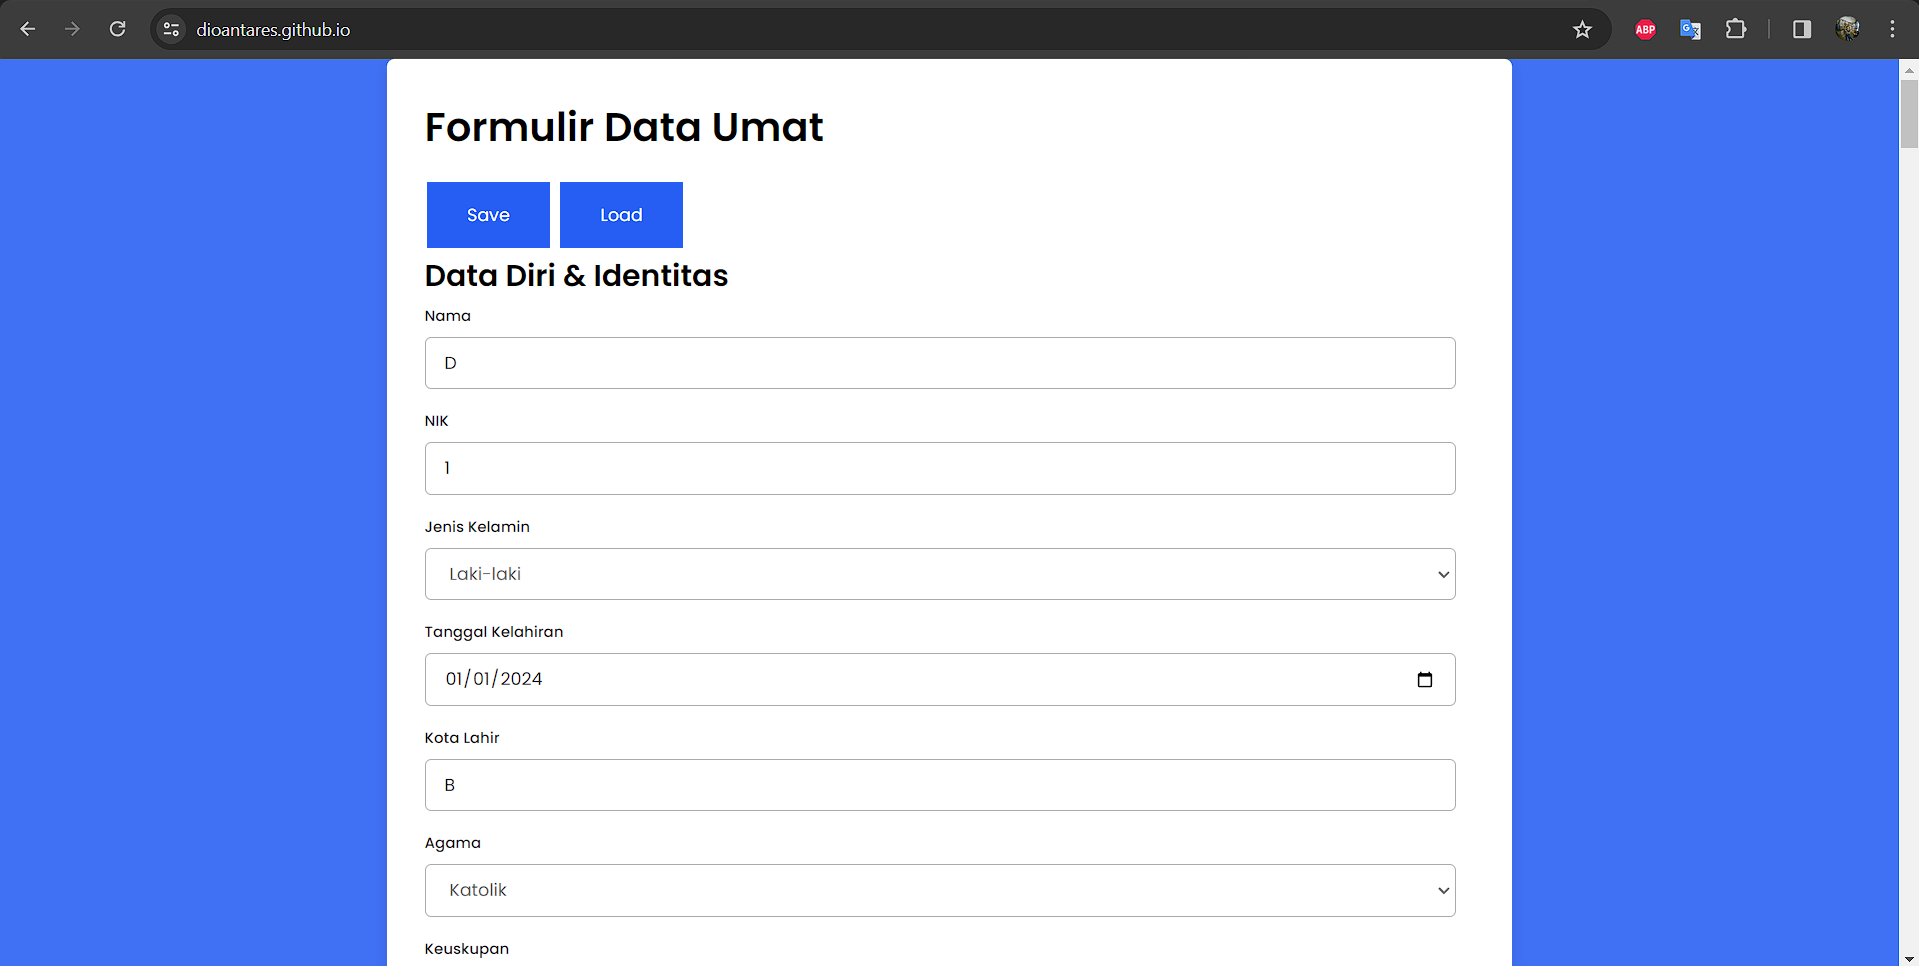
\includegraphics[scale=0.4]{Gambar/inputBestCase.png}
	\caption{Input data best case pada data formulir} 
	\label{fig:inputBestCase}
\end{figure}

\begin{figure}[H]
	\centering
	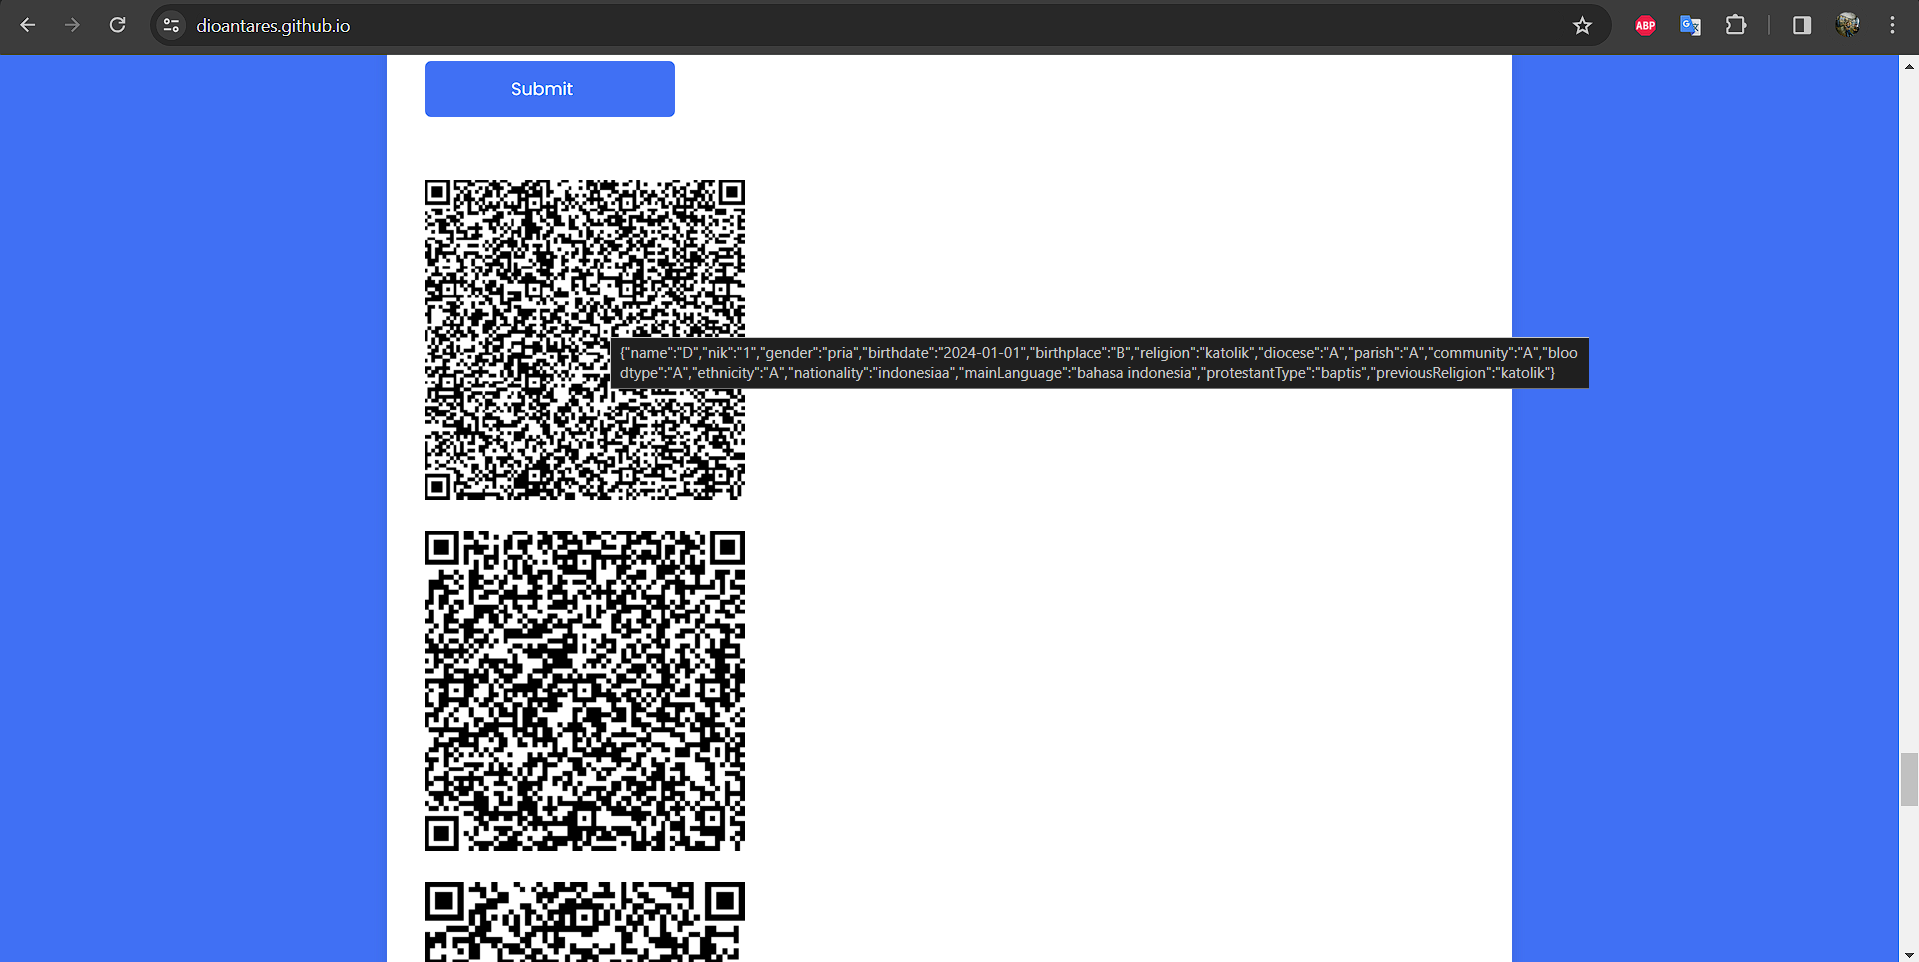
\includegraphics[scale=0.4]{Gambar/qrCodeBestCase.png}
	\caption{Hasil qr code best case dari data formulir} 
	\label{fig:qrCodeBestCase}
\end{figure}

\begin{figure}[H]
	\centering
	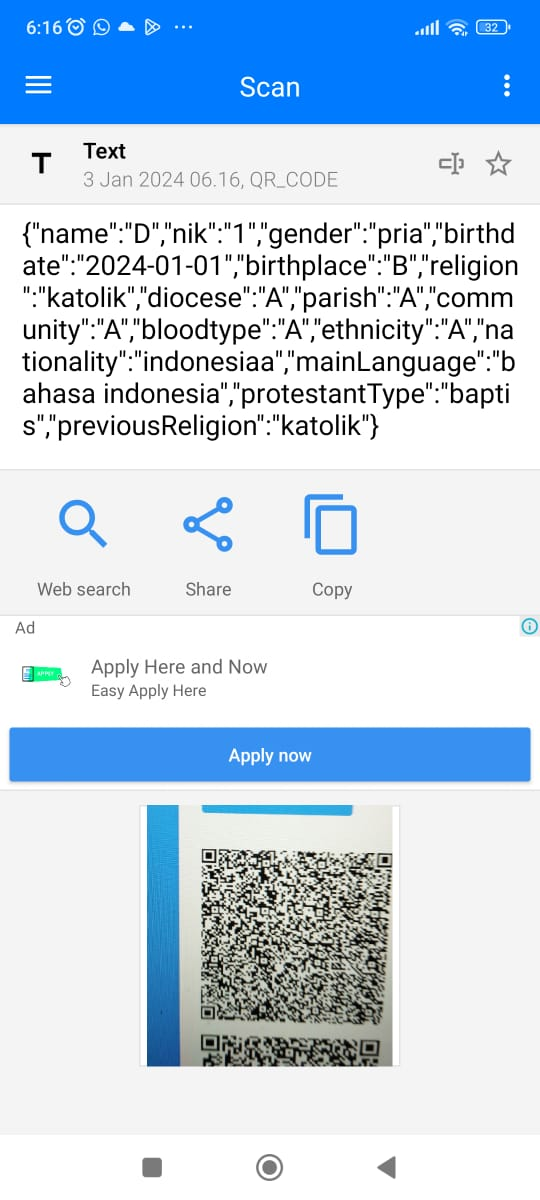
\includegraphics[scale=0.4]{Gambar/hasilScanBest.jpg}
	\caption{Hasil scan QR Code melalui aplikasi pada handphone} 
	\label{fig:hasilScanBest}
\end{figure}

Hasil pengujian ini mendapatkan hasil yang bagus, terbukti pada gambar \ref{fig:hasilScanBest}, qr code terlihat sangat jelas karena hanya berisikan satu huruf data input saja.

\subsection{Pengujian Worst Case}
\label{sec:pengujianWorst}

Pada pengujian kali ini, akan dimasukan data yang berisikan tulisan yang panjang, pada pengujian ini bertujuan untuk melihat apakah Qr Code yang dihasilkan dapat dipindai atau tidak, contoh input data yang dimasukkan dapat dilihat pada gambar \ref{fig:inputWorstCase}.

\begin{figure}[H]
	\centering
	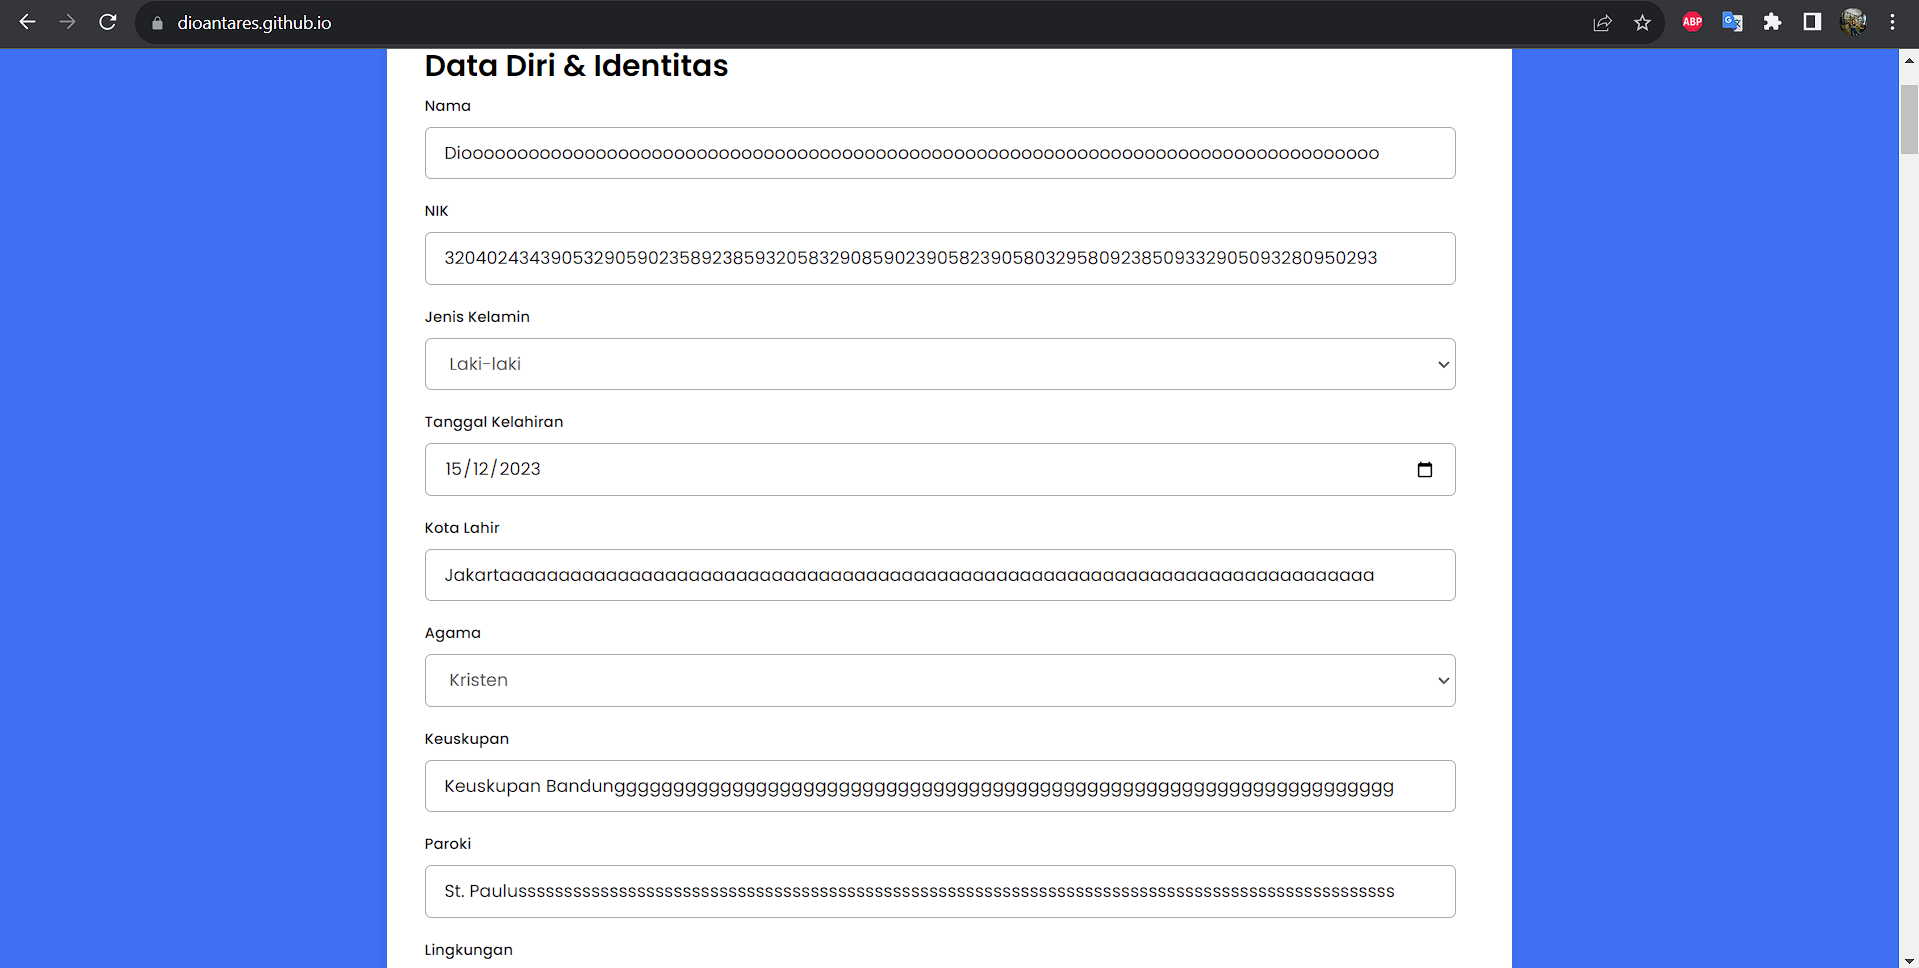
\includegraphics[scale=0.4]{Gambar/inputWorstCase.png}
	\caption{Input data worst case pada data formulir} 
	\label{fig:inputWorstCase}
\end{figure}

\begin{figure}[H]
	\centering
	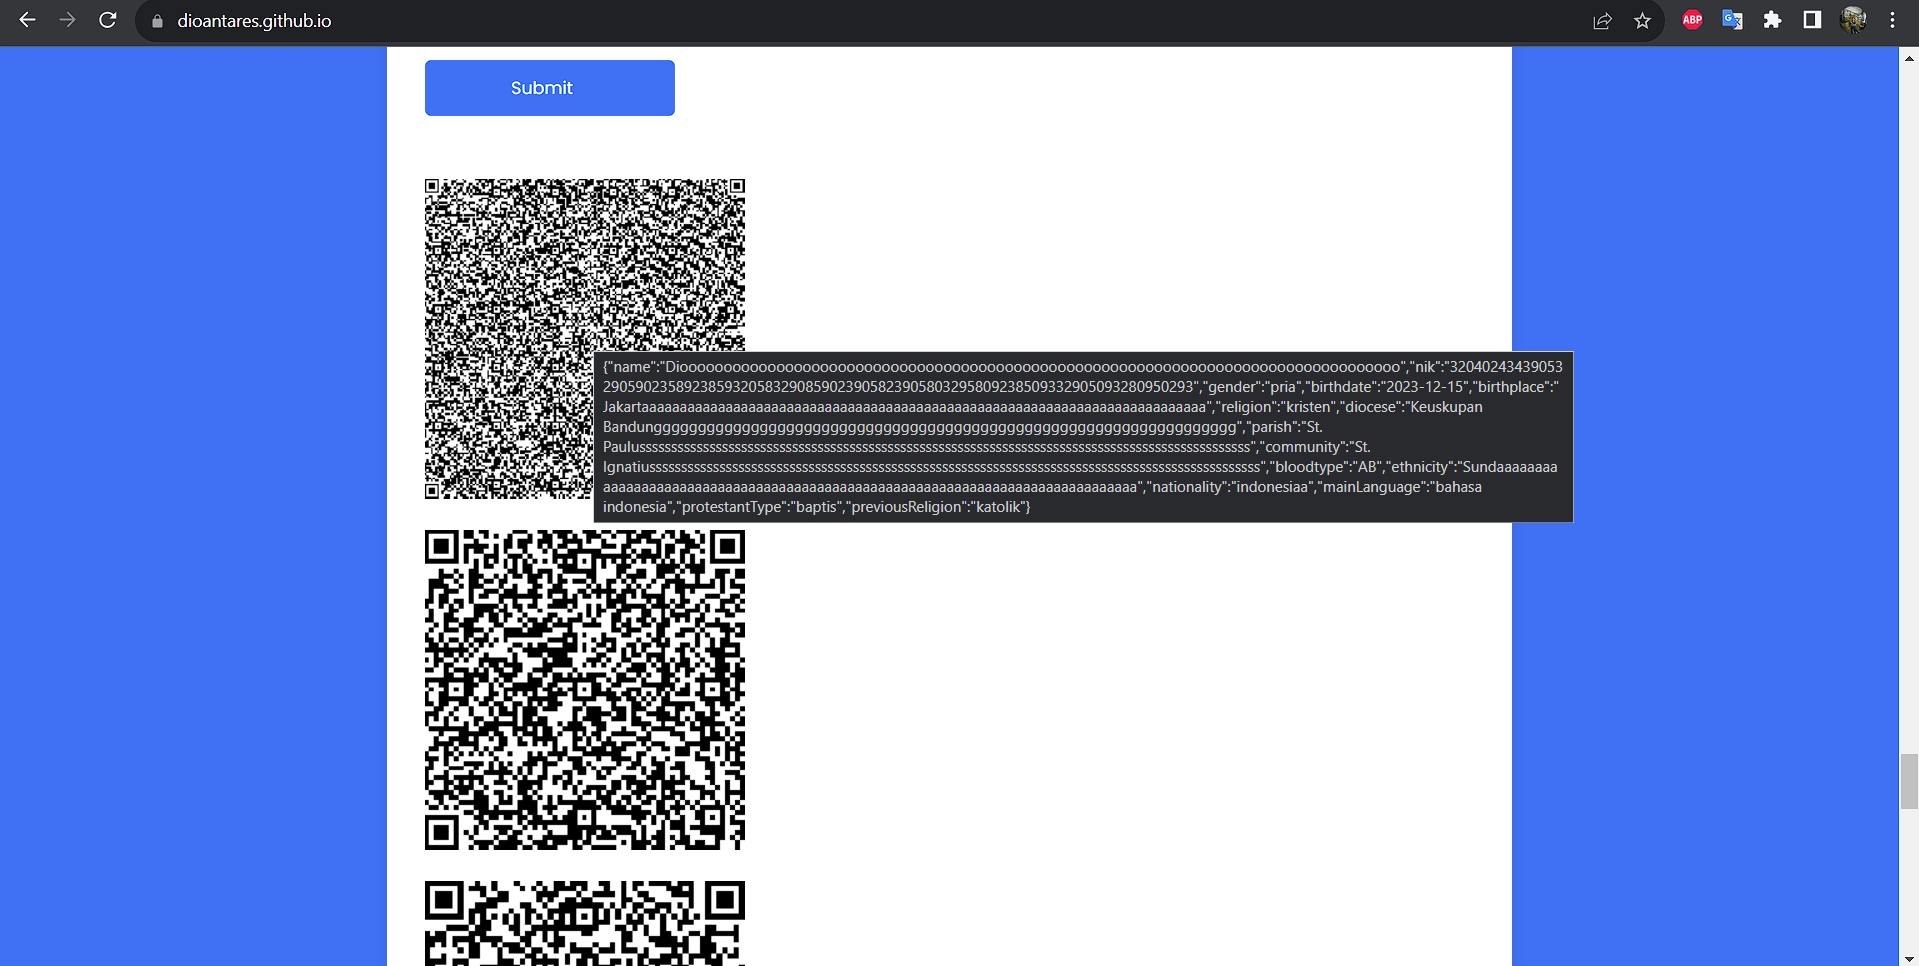
\includegraphics[scale=0.4]{Gambar/qrCodeWorstCase.png}
	\caption{Hasil qr code worst case dari data formulir} 
	\label{fig:qrCodeWorstCase}
\end{figure}

\begin{figure}[H]
	\centering
	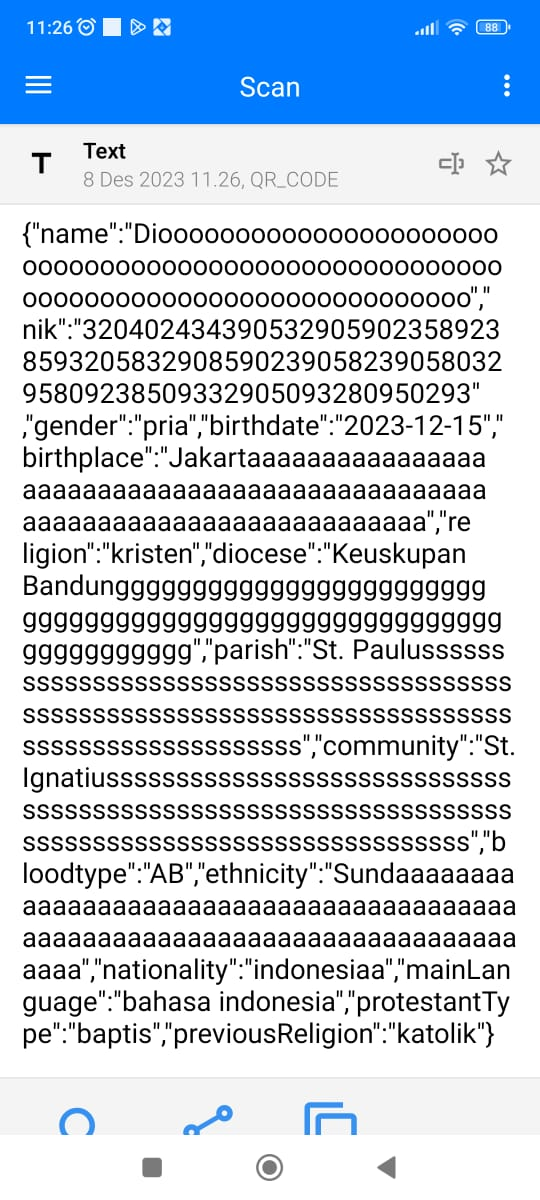
\includegraphics[scale=0.4]{Gambar/hasilScanWorst.jpg}
	\caption{Hasil scan QR Code melalui aplikasi pada handphone} 
	\label{fig:hasilScanWorst}
\end{figure}

Apabila data yang dimasukkan seperti pada gambar \ref{fig:inputWorstCase}, walaupun QR Code yang dihasilkan sangat kecil, dan hampir tidak bisa dipindai, namun setelah dilakukan pengujian, data tersebut masih dapat dipindai, hasil dari QR Code tersebut dapat dilihat pada gambar \ref{fig:hasilScanWorst}, namun QR Code memerlukan waktu yang lebih lama untuk dipindai dikarenakan QR Code berisikan banyak data.





